\documentclass{book}

\usepackage[utf8]{inputenc}
\usepackage{titlesec}
\usepackage{easylist}
\usepackage{hanging}
\usepackage{hyperref}
\usepackage[a4paper,top=2.0cm,bottom=2.0cm,left=2.0cm,right=3.0cm]{geometry}
\usepackage{blindtext}
\usepackage{tipa}
\usepackage{epigraph}
\usepackage{enumerate}
\usepackage{longtable}
\usepackage{setspace}
\usepackage{verbatim}
\usepackage[T1]{fontenc}
\usepackage{graphicx}
\usepackage[italian]{babel}
\usepackage{amsmath}
\usepackage{pbox}
\usepackage{fancyhdr}
\usepackage{cancel}
\usepackage{tabularx}
\usepackage{booktabs}
\usepackage{multirow}
\usepackage{longtable}
\usepackage{tikz}
\usepackage{tikz-qtree}
\usepackage{subfig}
\usepackage{xcolor}
\usepackage{amssymb}
\usepackage{mathrsfs}
\usepackage{textcomp}
\usepackage{circuitikz}
\usepackage{pifont}
\usepackage{imakeidx}
\usepackage{verbatim}
\usepackage{dsfont}
\usepackage{listings}
\usepackage{color}
\usepackage{upgreek}


\definecolor{mygreen}{rgb}{0,0.6,0}
\definecolor{mygray}{rgb}{0.5,0.5,0.5}
\definecolor{mymauve}{rgb}{0.58,0,0.82}

\lstset{ 
  backgroundcolor=\color{white},   % choose the background color; you must add \usepackage{color} or \usepackage{xcolor}; should come as last argument
  basicstyle=\footnotesize,        % the size of the fonts that are used for the code
  breakatwhitespace=false,         % sets if automatic breaks should only happen at whitespace
  breaklines=true,                 % sets automatic line breaking
  captionpos=b,                    % sets the caption-position to bottom
  commentstyle=\color{mygreen},    % comment style
  deletekeywords={...},            % if you want to delete keywords from the given language
  escapeinside={\%*}{*)},          % if you want to add LaTeX within your code
  extendedchars=true,              % lets you use non-ASCII characters; for 8-bits encodings only, does not work with UTF-8
  firstnumber=1000,                % start line enumeration with line 1000
  frame=single,	                   % adds a frame around the code
  keepspaces=true,                 % keeps spaces in text, useful for keeping indentation of code (possibly needs columns=flexible)
  keywordstyle=\color{blue},       % keyword style
  language=Octave,                 % the language of the code
  morekeywords={*,...},            % if you want to add more keywords to the set
  numbers=left,                    % where to put the line-numbers; possible values are (none, left, right)
  numbersep=5pt,                   % how far the line-numbers are from the code
  numberstyle=\tiny\color{mygray}, % the style that is used for the line-numbers
  rulecolor=\color{black},         % if not set, the frame-color may be changed on line-breaks within not-black text (e.g. comments (green here))
  showspaces=false,                % show spaces everywhere adding particular underscores; it overrides 'showstringspaces'
  showstringspaces=false,          % underline spaces within strings only
  showtabs=false,                  % show tabs within strings adding particular underscores
  stepnumber=2,                    % the step between two line-numbers. If it's 1, each line will be numbered
  stringstyle=\color{mymauve},     % string literal style
  tabsize=2,	                   % sets default tabsize to 2 spaces
  title=\lstname                   % show the filename of files included with \lstinputlisting; also try caption instead of title
}

\linespread{1.2} % l'interlinea

\frenchspacing

\newcommand{\abs}[1]{\lvert#1\rvert}

\usepackage{floatflt,epsfig}

\usepackage{multicol}
\newcommand\yellowbigsqcup[1][\displaystyle]{%
  \fboxrule0pt
  \ifx#1\textstyle\fboxsep-0.6pt\else\fboxsep-1.25pt\fi
  \mathrel{\fcolorbox{white}{yellow}{$#1\bigsqcup$}}}

\title{Appunti di Matematica}
\author{Nicola Ferru}
\date{}
\makeindex[columns=3, title=Alphabetical Index, intoc]

\begin{document}
\maketitle
\tableofcontents
\listoftables
\listoffigures

\section{Premesse\dots}

In questo repository, inoltre,  sono disponibili le dimostrazioni grafiche realizzate
con \textit{Geogebra}; consiglio a tutte le persone che usufruiranno di questo lavoro, di dare un occhiata alle dimostrazioni grafiche e stare attenti,  in quanto nel tempo potranno  essere presenti delle modifiche, cosi da apportare miglioramenti al contenuto degli stessi appunti.  Solitamente il lavoro di revisione viene fatto tre/quattro volte alla settimana perché sono in piena fase di sviluppo.  Ricordo a tutti che essendo un progetto volontario ci potrebbero essere dei rallentamenti per cause di ordine superiore e quindi
potrebbero esserci meno modifiche del solito oppure essere presenti degli errori.  Chiedo pertanto  la cortesia a voi lettori di contattarmi per apportare eventuali correzioni .  Tengo a precisare che tutto il progetto è puramente open source, pertanto vengono resi disponibili i sorgenti dei file LaTex  insieme ai PDF compilati.

\begin{center}
	Cordiali saluti
\end{center}
\newpage

\section{Simboli}
\begin{multicols}{3}
	$\in$ Appartiene\\
	$\notin$ Non appartiene\\
	$\exists$ Esiste\\
	$\exists !$ Esiste unico\\
	$\subset$ Contenuto strettamente\\
	$\subseteq$ Contenuto\\
	$\supset$ Contenuto strettamente\\
	$\supseteq$ Contiene\\
	$\Rightarrow$ Implica\\
	$\Longleftrightarrow$ Se e solo se\\
	$\neq$ Diverso\\
	$\forall$ Per ogni\\
	$\ni :$ Tale che\\
	$\leq$ Minore o uguale\\
	$\geq$ Maggiore o uguale\\
	$\alpha$ alfa\\
	$\beta$ beta\\
	$\gamma$ gamma\\
	$\Gamma$ Gamma\\
	$\delta,\Delta$ delta\\
	$\epsilon$ epsilon\\
	$\sigma,\Sigma$ sigma\\
	$\rho$ rho
\end{multicols}

\part{Matematica analisi 1}
\chapter{Cenni di teoria degli insiemi}
Per rappresentare un insieme abbiamo tre possibilità:
\begin{enumerate}
	\item Rappresentazione estensive $A=[0,1,2,3,4]$
	\item Rappresentazione intensiva $A=[x|x\in N e x<5]$
	\item Rappresentazione con diagrammi di Eulero - Venn\\
	\begin{tikzpicture}domain=0:10] 
		 \draw (0,0) ellipse (2cm and 1cm);
    		 \filldraw  (0,0.3) circle (2pt) node[align=left,   below] {1}
    			(1,0.11) circle (2pt) node[align=left,   below] {2}
    			(-1,-0.4) circle (2pt) node[align=left,   below] {0}
    			(-1,0.1) circle (2pt) node[align=left,   below] {3}
    			(0.1,-0.5) circle (2pt) node[align=left,   below] {4};
		\end{tikzpicture}
\end{enumerate}
\subsection{Operazioni tra gli insiemi}
Un insieme può essere contenuto in un altro:\\
\begin{tikzpicture}domain=0:10] 
    \draw (0,0) ellipse (2cm and 1cm);
     \draw (0,0) ellipse (0.7cm and 0.5cm);

    \filldraw  (0,0.3) circle (2pt) node[align=left,   below] {1}
    (-0.52,0.3) node[align=left,   below] {B}
    (0.55,0.11) circle (2pt) node[align=left,   below] {2}
    (-1,-0.4) circle (2pt) node[align=left,   below] {0}
    (-1,0.1) circle (2pt) node[align=left,   below] {3}
    (0.6,-0.55) circle (2pt) node[align=left,   below] {4};
\end{tikzpicture}
\section{Sottoinsiemi di R}
\subsection{Definizione}
\begin{enumerate}
	\item Un punto $x_0$ si dice intero ad A se esiste un suo interno I($x_0,\delta$)
con $\delta>0$ contenuto in A.
	\item Si dice esterno ad A se è interno al CA ($A^c$).
	\item Si dice di frontiera per A se non è né interno né esterno ad A.
\end{enumerate}
\subsubsection{Interno di A}
\paragraph{°A} Insieme dei punti interni ad A.
\paragraph{Esempio} se $A=(1,3],\text{ }A=(1,3)$
\paragraph{$\partial$A,FA} Insieme dei punti di frontiera di A
\paragraph{Esempio} se $A=(1,3]$, i punti di frontiera sono i punti $x=1$ e
$x=3$
\subsubsection{Osservazioni}
\begin{itemize}
	\item Se $x_0\in {^\circ A}\Rightarrow x_0\notin A$
	\item Se $x_0\notin {^\circ A} \text{ (esterno)} \Rightarrow x_0\notin A$
	\item Se $x_0\in\partial A \text{ (frontiera) può essere }x_0\in A \text{
			oppure} x_0 \notin A, \text{ in ogni caso per} \forall
		I(x_0.\delta) $ continue sia punti di A sia punti CA.
\end{itemize}
\paragraph{Definizione}
$x_0$ è un punto di accumulazione per A se in $\forall I(x_0,\delta)$ esiste un
punti di A diverso da $x_0$. (Cioè in ogni interno di $x_0 \exists$ infiniti
elementi di A)
\subparagraph{Esempio} se $A=(-2,3],x=-2$ è accumulazione per A, ma anche
$x=3,x=0,x=1,\dots$, cioè è di accumulazione per A, qualunque $x\in [2,3]$.\\
DA=A'=derivato di A è l'insieme dei punti di accumulazione per A. Se $x_0\in
DA$ allora può aversi $x_0\in A$ oppure $x_0\notin A$
\paragraph{Esercizio} $x=1 \text{e} x=3$ sono entrambi punti di accumulazione
per l'intervallo $(1.3],x=3$ appartiene all'intervallo dato, x=1 NO.
\begin{enumerate}
	\item Se $x_0\in A \Rightarrow x_0\in DA$;
	\item Se $x\notin DA$ allora $x_0$ si dice isolato;
	\item Se $DA=\phi\Rightarrow$ A si dice discreto \textbf{Esempio}
		$A=\{1,2,3,4\}$
	\item Se $DA=A\Rightarrow A$ si dice perfetto \textbf{Esempio} $A=[a,b]$
\end{enumerate}
\paragraph{Definizione}
Dato $A\subset R$ si definisce chiusura di A e si indica con $\bar{A}$,
l'insieme:
\begin{tabular}{|c|}
	\hline
	$\bar{A}=A\bigcup \partial A$\\
	\hline
\end{tabular} A è chiuso $\Leftrightarrow A=\bar{A}$
\paragraph{Esempio} se $A=(2,5]$, allora $\bar{A}=[2,5]$
\subsubsection{Teorema di Bolzano Weierstrass}
Ogni $A\subset R^n$ limitato e finito possiede almeno un punto di
accumulazione. Un insieme chiuso e limitato in $R^n$ ammette massimo e minimo
assoluto.
\paragraph{Esempio} $A=[1,4],\text{ } max(A)=4,\text{ } min(A)=1 \text{ }
A=\{x\in R:x^2\leq 1\} \text{ } max{A}=1, \text{ } min(A)=-1$
\section{Funzione di una variabile}
\subsection{Definizione}
Dati A, $B\subseteq R$ una funzione A in B è una legge (o relazione, o mappa)
che ad ogni elemento x di A associa uno ed un solo elemento y di B.
\textit{f}: $A\to B$ oppure $y=f(x)$ $x\in A$ e $y=f(x)\in R$
\begin{itemize}
	\item A = dominio o insieme di definizione di f.
	\item B = codominio di f.
\end{itemize}
\begin{figure}[!ht]
	\begin{tikzpicture}

	\end{tikzpicture}

\end{figure}
Il grafico di f è un insieme di punti del piano (generalmente una curva) che è
sottoinsieme del prodotto cartesiano AxB costituito da (x, f(x)) con $x\in A,
f(x)\in B$
\paragraph{Definizione di funzione Immagine}
L'immagine di A tramite f, f(A), è l'insieme dei valori di y tale che $\exists
x \in A$ tale che $f(x) \in B$.
\subparagraph{Esempio} Se \textit{f}: $A\to B$ $f(x)=x^2 \text{ } A=R,
f(A)=[0,+\infty)$\\
\paragraph{Definizione di funzione suriettiva} Si dice che \textit{f}: $A\to B$
è suriettiva se $f(A)=B$ (cioè fissato $y\in B \exists x\in A: y=f(x)$)
\paragraph{Definizione di funzione iniettiva}
Si dice che \textit{f}: $A\to B$ è iniettiva se $x_2\neq x_1\Rightarrow f(x_1)
\neq f(x_2)$
\paragraph{Una funzione può essere sia iniettiva che suriettiva ``biiettiva''}
Se \textit{f} è sia suriettiva che iniettiva allora si dice biiettiva (\textbf{cioè si
ha un corrispondenza biunivoca tra A e B})
\paragraph{Quando una funzione è pari?}
Una funzione è pari se $\forall x\in A: f(x)=f(-x)$ quindi il grafico di
\textit{f} è simmetrico rispetto all'asse Y (es. $y=x^2$)
\paragraph{Quando una funzione è dispari?}
Una funzione è dispari se $\forall x\in A: f(-x)=-f(-x), f(x)=-f(-x)$ quindi il
grafico di \textit{f} è simmetrico rispetto all'origine (es. $y=x^3$)
\paragraph{Quando una funzione è periodica?}
Una funzione $A\to B$ è periodica di periodo $T>0$, se $\forall x \in A, x+T\in
A \text{ e } f(x+T)=f(x)$ 
\subparagraph{Esempio} Funzioni trigonometriche
\paragraph{Quando una funzione è limitata superiormente?}
Una funzione si dice limitata superiormente se $\exists M\in R: f(x)\leq M$
$\forall x \in A$ (il grafico di \textit{f} sta sotto la retta orizzontale $y=m$)
\paragraph{Quando una funzione è limitata inferiormente?}
Analogamente, al caso precedente, una funzione si dice limitata inferiormente
se $\exists m\in R:f(x)\leq m \forall x \in A$ (il grafico di \textit{f} sta
sopra la retta orizzontale $y=m$. La funzione f si dirà limitata se è limitata
sia inferiormente che superiormente).
\paragraph{Quando una funzione viene definita \textit{composta}?}
Una funzione $A\to B \text{ e } B\to C$ si definisce composta di \textit{f} e
\textit{g}: $g(f(x))$ La funzione \textit{h}: $A\to C h=g^of$
\subparagraph{Esempio} \textit{f}=$x^2,g(x)=3x+2, \text{ } (A \equiv B \equiv C
\equiv R) g^of=3x^2+2$
\subparagraph {Esempio}
\textit{f}=$x^2,g(x)=3x+2$
\begin{figure}[!ht]
	\centering
	\begin{tikzpicture}
		\node[] (pic) at (0,0) {\includegraphics[height=8cm]{img/insiemi funzioni
			composte.pdf}};
	\end{tikzpicture}
	\caption{Grafico di insieme di \textit{f}=$x^2,g(x)=3x+2$}
\end{figure}\\
\begin{tabular}{|l|}
	\hline
		$g^of=3x^2+2$\\
	\hline
\end{tabular}\\
L'operazione di composizione non è commutativa ($g^of\neq f^og$). La
composizione di due funzioni biiettive è biiettiva
\paragraph{Quando una funzione è inversa?}
Date \textit{f}: $A\to B$ biiettiva, si definisce funzione inversa di
\textit{f}: $f^{-1}:_B\to A$ tale che $f^{-1}$ o $f=I_A$ \textit{f} o
$f^{-1}=I_B$
\paragraph{Nota} La funzione $y=x^2$ (\textit{f}: $R\to R$) non è biiettiva ma
è stata ``resa'' biiettiva, quindi invertibile, restringendo il suo dominio
(per l'iniettività) e codominio (per la suriettività). Nell'esempio il dominio
è stato <<rimpicciolito>> in modo tale da avere una funzione strettamente
crescente e quindi iniettiva. Il codominio è stata <<rimpicciolito>>
all'intervallo massimale $[0,+\infty)$ e la funzione è diventata anche
suriettiva.
\paragraph{Quando una funzione viene definita monotona?}
Sia \textit{f}:$A\to B$, f si dice monotona in A se verifica una delle seguenti
condizioni ($\forall x_1,x_2\in A$)
\begin{enumerate}
	\item \textit{f} strettamente crescente se $x_1<x_2$, $f(x_1)<f(x_2)$
	\item \textit{f} crescente se $x_1<x_2$, $f(x_1)\leq f(x_2)$
	\item \textit{f} strettamente decrescente se $x_1<x_2$, $f(x_1)<f(x_2)$
	\item \textit{f} decrescente se $x_1<x_2$, $f(x_1)\geq f(x_2)$
\end{enumerate}
\fbox{
 	\addtolength{\linewidth}{-2\fboxsep}%
 	\addtolength{\linewidth}{-2\fboxrule}%
 	\begin{minipage}{\linewidth}
		\textit{Se si verificano la 1 e 3 allora la funzione f(x) è {\color{red}
			strettamente monotona.}}
		\paragraph{Teorema:} \textit{Una funzione f:$A\to B$ strettamente monotona in A, è
		invertibile in A. Inoltre la sua inversa è ancora strettamente monotona.}
	\end{minipage}
}

\chapter{Studio di funzione}
\texttt{In analisi matematica la locuzione studio di funzione indica 
	l'applicazione pratica dei teoremi e delle tecniche del calcolo 
	infinitesimale nello specifico caso di una funzione di cui è nota 
	l'espressione analitica. Lo studio di funzione è utile per ricavare 
	esplicitamente le informazioni che descrivono il comportamento di una 
	funzione nel suo dominio. Spesso, le informazioni ottenute mediante uno 
	studio di funzione sono sufficienti per poter tracciare, anche a mano, un 
	grafico qualitativo della funzione studiata e che in genere, per funzioni a 
	valori reali di una variabile reale, viene rappresentato su un piano 
	cartesiano, anche se in taluni casi potrebbe essere più semplice ricorrere 
	un sistema di coordinate differente. In genere, con "studio di funzione" ci 
	si riferisce implicitamente al solo e specifico caso delle funzioni reali di
	una sola variabile reale, ma con le opportune modifiche è comunque possibile 
	adattare le considerazioni seguenti anche al caso delle funzioni di più
	variabili reali, nonché anche per le funzioni di una o più variabili 
	complesse.}
\begin{center}
	By \href{https://it.wikipedia.org/wiki/Studio_di_funzione}{Wikipedia}
\end{center}

\section{Grafica delle funzioni elementari}
\subsection{Funzione lineare $y=mx+qm, q\in R$}
\begin{figure}[!ht]
	\centering
	\begin{tikzpicture}
		\node[] (pic) at (0,0) {\includegraphics[height=8cm]{img/funzione
		lineare.pdf}};
	\end{tikzpicture}
	\caption{Grafico di Funzione lineare $y=mx+qm, q\in R$}
\end{figure}
$C.E. \equiv R\text{ Non Limitata}$
\subsection{Funzione valore assoluto $y=|x|$}
\begin{figure}[!ht]
	\centering
	\begin{tikzpicture}
		\node[] (pic) at (0,0) {\includegraphics[height=8cm]{img/funzione valore assoluto.pdf}};
	\end{tikzpicture}
	\caption{Grafico di Funzione valore assoluto $y=|x|$}
\end{figure}
$C.E. \equiv R\text{ Limitata inferiormente in } x=0$\\
$|x|=\begin{cases}
	x&x\geq0\\
	-x& x<0
\end{cases}$
\subsection{Funzione potenza $y=x^n,n\in N, pari$}
\begin{figure}[!ht]
	\centering
	\begin{tikzpicture}
		\node[] (pic) at (0,0) {\includegraphics[height=8cm]{img/funzione
		potenziale x^n.pdf}};
	\end{tikzpicture}
	\caption{Grafico di Funzione potenza $y=x^n,n\in N, pari$}
\end{figure}\newpage
\subsection{Funzione potenza $y=x^\alpha,\alpha \in R$ (\textit{ma non
razionale})}
\begin{figure}[!ht]
	\centering
	\begin{tikzpicture}
		\node[] (pic) at (0,0) {\includegraphics[height=8cm]{img/funzione
		potenziale x^a.pdf}};
	\end{tikzpicture}
	\caption{Grafico di Funzione potenza $y=x^\alpha,\alpha \in R$ (\textit{ma non
razionale})}
\end{figure}
$C.E.:\{x\in R: x\geq 0\}$ Limitata inferiormente da $x=0$ non limitata
superiormente Strettamente crescente
\subsection{Funzione potenziale $y=x^{\frac{m}{n}},m, n\in Z$}
\begin{figure}[!ht]
	\centering
	\begin{tikzpicture}
		\node[] (pic) at (0,0) {\includegraphics[height=8cm]{img/funzione
		potenziale fratta.pdf}};
	\end{tikzpicture}
	\caption{Grafico di Funzione potenza $y=x^\alpha,\alpha \in R$ (\textit{ma non
razionale})}
\end{figure}
\subsection{Funzione logaritmo $y=\log_a{x}$}
\begin{figure}[!ht]
	\centering
	\begin{tikzpicture}
		\node[] (pic) at (0,0) {\includegraphics[height=8cm]{img/funzione
		logaritmica.pdf}};
	\end{tikzpicture}
	\caption{Funzione logaritmo $y=\log_a{x}$}
\end{figure}
$C.E.\equiv x>0$ Non limitata, strettamente crescente se $a>1$, Strettamente
decrescente se $0<a<1$.\newpage
\subsection{Le coniche: la circonferenza}
\begin{figure}[!ht]
	\centering
	\begin{tikzpicture}
		\node[] (pic) at (0,0) {\includegraphics[height=8cm]{img/le coniche
		circonferenze.pdf}};
	\end{tikzpicture}
	\caption{Le coniche: la circonferenza}
\end{figure}\newpage
\subsection{Le coniche: l'ellisse}
\begin{figure}[!ht]
	\centering
	\begin{tikzpicture}
		\node[] (pic) at (0,0) {\includegraphics[height=8cm]{img/le coniche
		ellisse.pdf}};
	\end{tikzpicture}
	\caption{Le coniche: l'ellisse}
\end{figure}
\subsection{Le coniche: iperbole}
\begin{figure}[!ht]
	\centering
	\begin{tikzpicture}
		\node[] (pic) at (0,0) {\includegraphics[height=8cm]{img/le coniche
		iperbole.pdf}};
	\end{tikzpicture}
	\caption{Le coniche: iperbole}
\end{figure}\newpage
\subsection{Le coniche: iperbole equilattera}
\begin{figure}[!ht]
	\centering
	\begin{tikzpicture}
		\node[] (pic) at (0,0) {\includegraphics[height=8cm]{img/le coniche
		iperbole equilattera.pdf}};
	\end{tikzpicture}
	\caption{Le coniche: iperbole equilattera}
\end{figure}
\subsection{Le coniche: parabola}
\begin{figure}[!ht]
	\centering
	\begin{tikzpicture}
		\node[] (pic) at (0,0) {\includegraphics[height=8cm]{img/le coniche
		parabola.pdf}};
	\end{tikzpicture}
	\caption{Le coniche: parabola}
\end{figure}\newpage
\subsection{Le funzioni trigonometriche}
Funzioni trigonometriche elementati:
$y=\sin x, y=cos x, y=\tan x, y=\cot x$\\
\textit{Relazioni fondamentali:} $(\sin x)^2+(\cos x)^2=1$, $\tan x=\frac{\sin
x}{\cos x}$, $\cot x=\frac{\cos x}{\sin x}$
\begin{figure}[!ht]
	\centering
	\begin{tikzpicture}
		\node[] (pic) at (0,0) {\includegraphics[height=8cm]{img/funzioni
		trigonometriche.pdf}};
	\end{tikzpicture}
	\caption{Le funzioni trigonometriche}
\end{figure}
\subsubsection{Funzione $\sin x$}
\begin{figure}[!ht]
	\centering
	\begin{tikzpicture}
		\node[] (pic) at (0,0) {\includegraphics[height=8cm]{img/funzione
		sin.pdf}};
	\end{tikzpicture}
	\caption{Funzione $\sin x$}
\end{figure}\newpage
\subsubsection{Funzione $\cos x$}
\begin{figure}[!ht]
	\centering
	\begin{tikzpicture}
		\node[] (pic) at (0,0) {\includegraphics[height=8cm]{img/funzione
		cos.pdf}};
	\end{tikzpicture}
	\caption{Funzione $\cos x$}
\end{figure}
\subsubsection{Funzione $\tan x$}
\begin{figure}[!ht]
	\centering
	\begin{tikzpicture}
		\node[] (pic) at (0,0) {\includegraphics[height=8cm]{img/funzione
		tg.pdf}};
	\end{tikzpicture}
	\caption{Funzione $\tan x$}
\end{figure}\newpage
\subsubsection{Funzione $\cot x$}
\begin{figure}[!ht]
	\centering
	\begin{tikzpicture}
		\node[] (pic) at (0,0) {\includegraphics[height=8cm]{img/funzione
		ctg.pdf}};
	\end{tikzpicture}
	\caption{Funzione $\cot x$}
\end{figure}
\subsection{Le funzioni trigonometriche inverse}
\subsubsection{Funzione $\arcsin x$}
\begin{figure}[!ht]
	\centering
	\begin{tikzpicture}
		\node[] (pic) at (0,0) {\includegraphics[height=8cm]{img/funzione
		arcsin.pdf}};
	\end{tikzpicture}
	\caption{Funzione $\arcsin x$}
\end{figure}\newpage
\subsubsection{Funzione $\arccos x$}
\begin{figure}[!ht]
	\centering
	\begin{tikzpicture}
		\node[] (pic) at (0,0) {\includegraphics[height=8cm]{img/funzione
		arccos.pdf}};
	\end{tikzpicture}
	\caption{Funzione $\arccos x$}
\end{figure}
\subsubsection{Funzione $\arctan x$}
\begin{figure}[!ht]
	\centering
	\begin{tikzpicture}
		\node[] (pic) at (0,0) {\includegraphics[height=8cm]{img/funzione
		arctg.pdf}};
	\end{tikzpicture}
	\caption{Funzione $\arctan x$}
\end{figure}\newpage
\subsubsection{Operazione sul grafico: traslazione della asse X}
\begin{figure}[!ht]
	\centering
	\begin{tikzpicture}
		\node[] (pic) at (0,0) {\includegraphics[height=8cm]{img/operazione sul
		grafico traslazione della asse x.pdf}};
	\end{tikzpicture}
	\caption{Operazione sul grafico: traslazione della asse X}
\end{figure}
\subsubsection{Operazione sul grafico: traslazione della asse Y}
\begin{figure}[!ht]
	\centering
	\begin{tikzpicture}
		\node[] (pic) at (0,0) {\includegraphics[height=8cm]{img/operazione sul
		grafico traslazione della asse y.pdf}};
	\end{tikzpicture}
	\caption{Operazione sul grafico: traslazione della asse Y}
\end{figure}\newpage
\subsubsection{Operazione sul grafico: contrazione e dilatazione in direzione verticale}
\begin{figure}[!ht]
	\centering
	\begin{tikzpicture}
		\node[] (pic) at (0,0) {\includegraphics[height=8cm]{img/contrazione e
		dilatazione in direzione verticale.pdf}};
	\end{tikzpicture}
	\caption{Operazione sul grafico: contrazione e dilatazione in direzione verticale}
\end{figure}
\subsubsection{Operazione sul grafico: contrazione e dilatazione in direzione
orizzontale}
\begin{figure}[!ht]
	\centering
	\begin{tikzpicture}
		\node[] (pic) at (0,0) {\includegraphics[height=8cm]{img/compressione e
		dilatazione in direzione orizzontale.pdf}};
	\end{tikzpicture}
	\caption{Operazione sul grafico: contrazione e dilatazione in direzione
	orizzontale}
\end{figure}\newpage
\subsubsection{Operazione sul grafico: $y=|f(x)|$}
\begin{figure}[!ht]
	\centering
	\begin{tikzpicture}
		\node[] (pic) at (0,0) {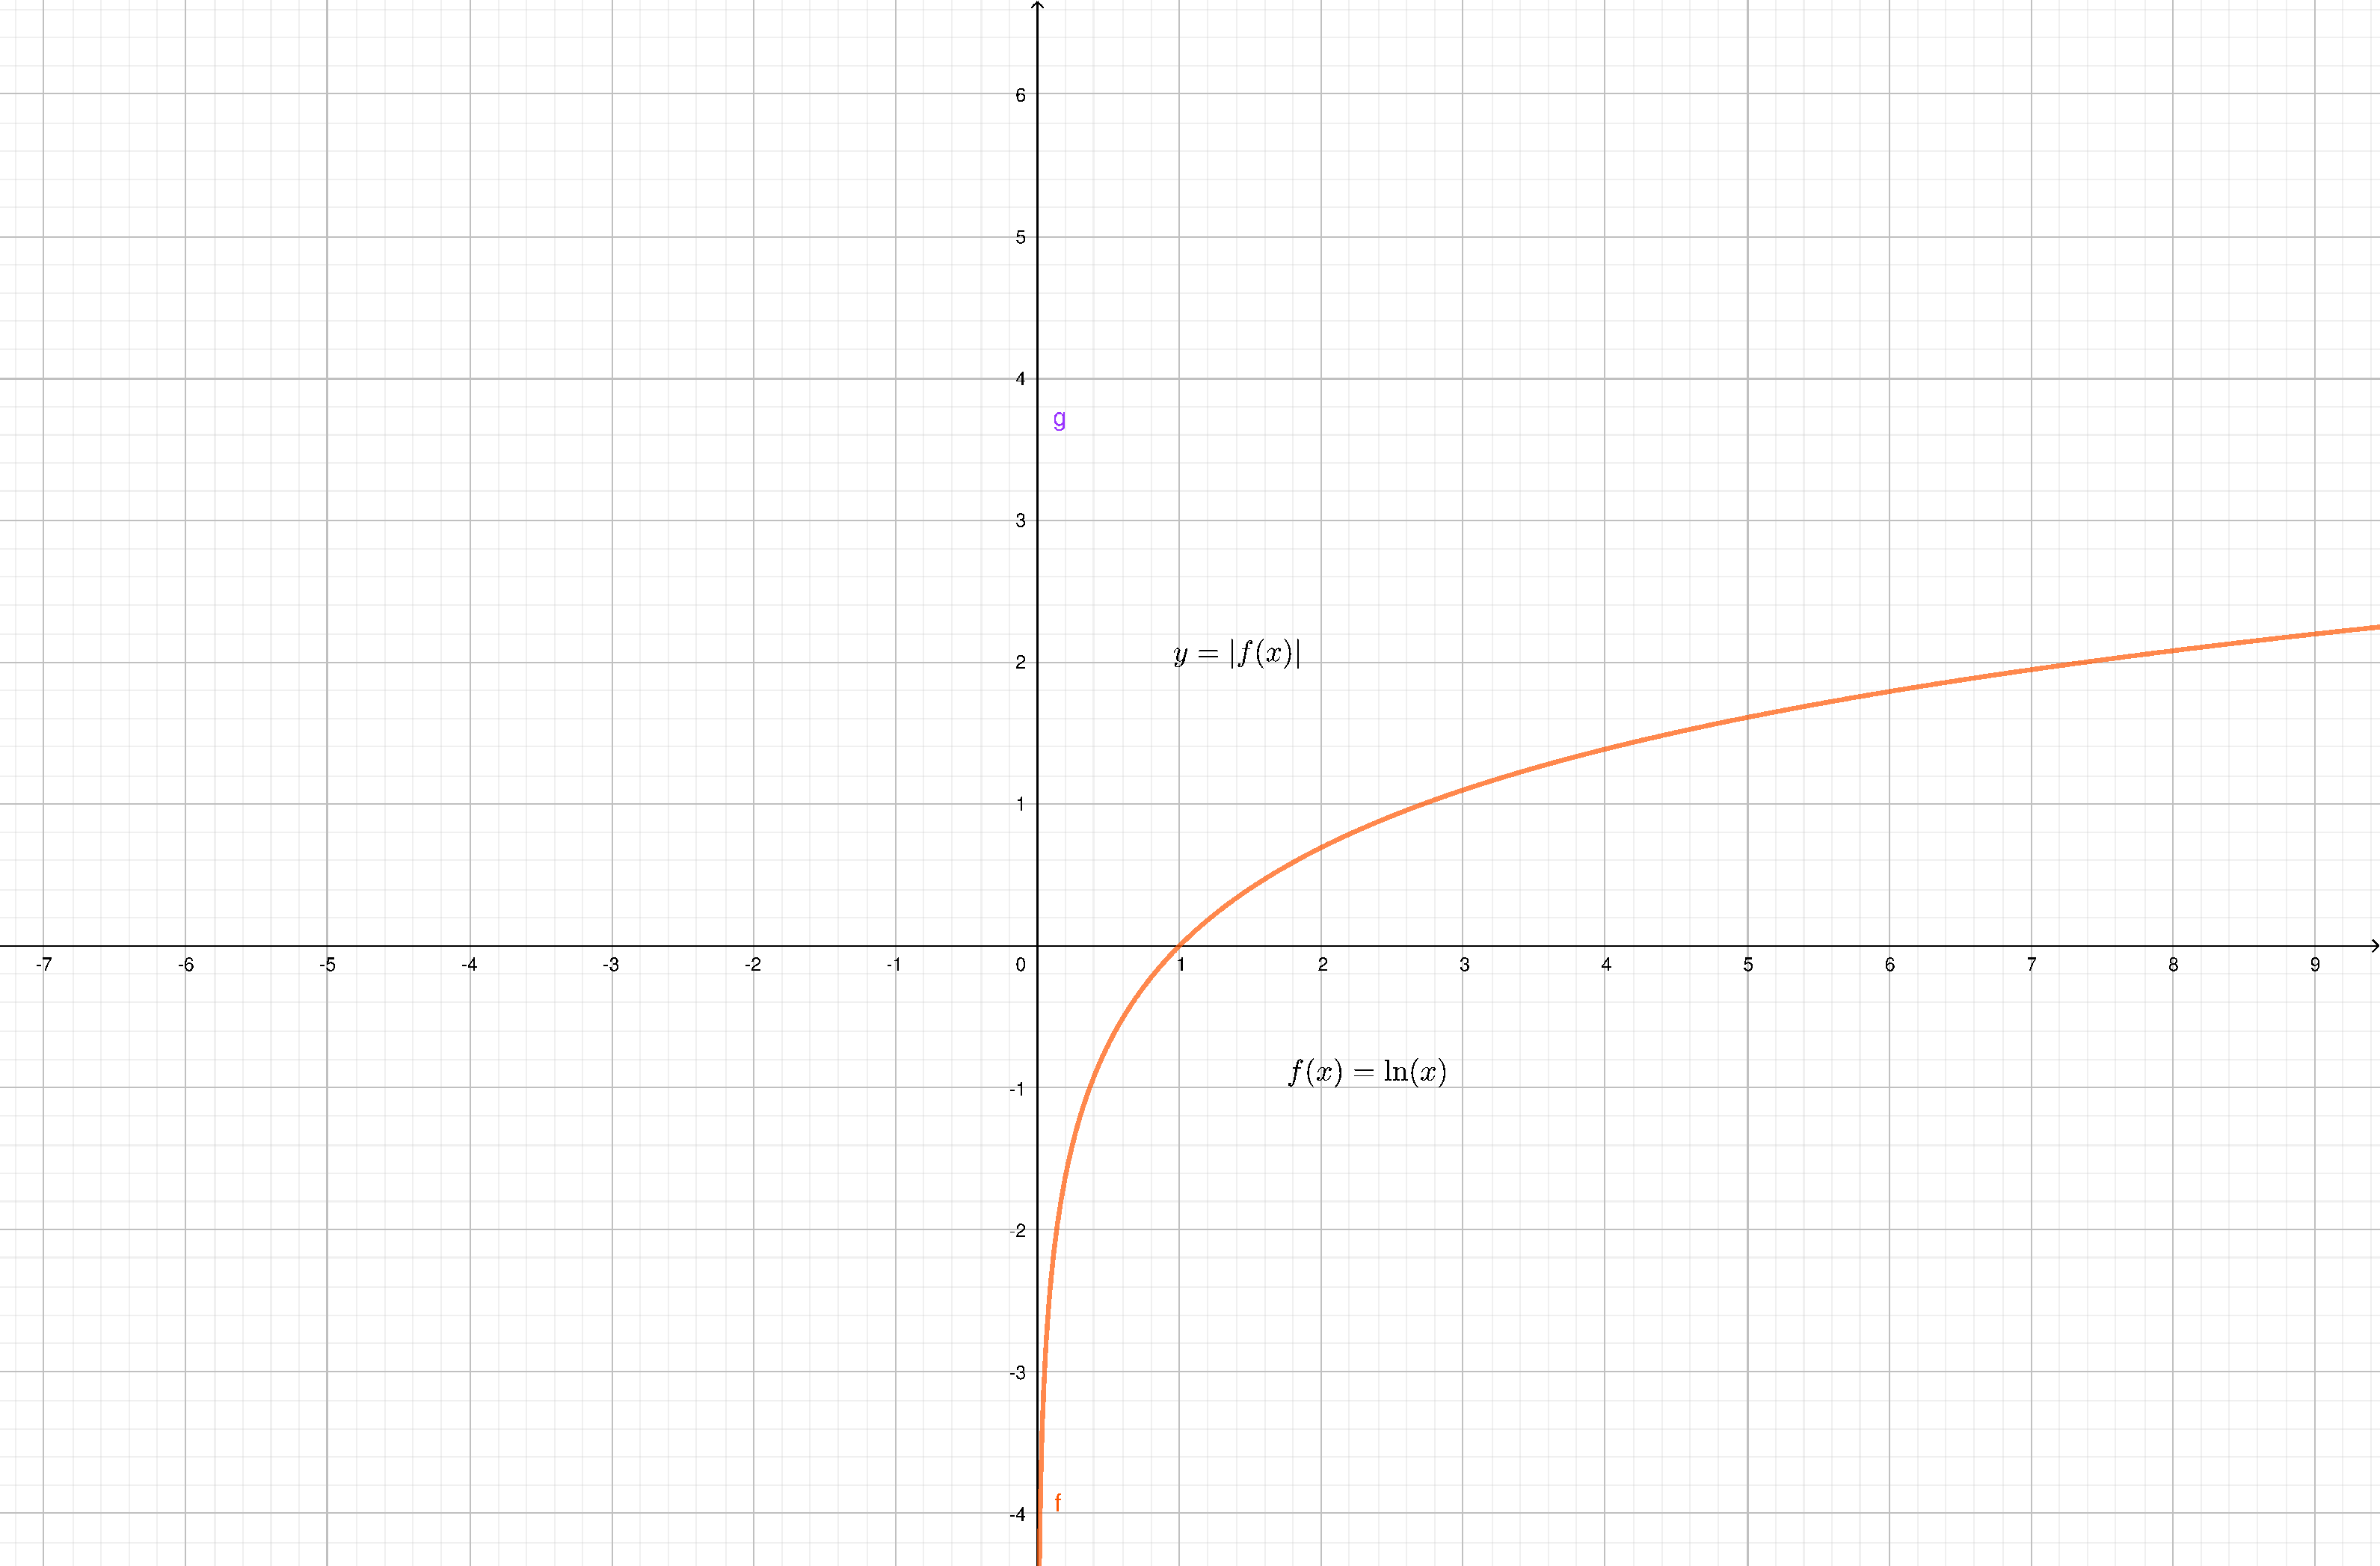
\includegraphics[height=8cm]{img/y=_lnx_.pdf}};
	\end{tikzpicture}
	\caption{Operazione sul grafico: $y=|f(x)|$}
\end{figure}



\begin{enumerate}
	\item Criterio di monotonia\\
		Sia $f(x):[a,b]\to R$, continue in $[a,b]$, è derivabile in $(a,b)$.
		Allora:
		\begin{itemize}
			\item f è crescente in $[a,b]\Leftrightarrow f^\prime(x)\geq 0
				\forall x \in [a,b]$;
			\item f è crescente in $[a,b]\Leftrightarrow f^\prime(x)\leq 0
				\forall x \in [a,b]$.
		\end{itemize}
		\paragraph{Dimostrazione}
		Sia $f^\prime (x)\geq 0 \text{ e siano } x_1,x_2\in[a,b]\text{ con }
		x_2>x_1$.\\
		Per il Teorema di Lagrange $\forall x_0\in (x_1,x_2)$:	
			\begin{center}
				$f(x_2)-f(x_1)=f^\prime(x_0)(x_2-x_1)$
			\end{center}
			ma $f^\prime(x_0)\geq 0$ e $x_2-x_1>0 \Rightarrow f(x_2)\geq f(x_1)$
		\paragraph{Viceversa} Sia $f(x)$ crescente in $[a,b]$.\\
		Allora $\forall x, x+h\in (a,b)$, si ha $\frac{f(x+h)-f(x)}{h}\geq 0$\\
		Facendo il limite per $h\to 0$ si ha
		\begin{center}
			$f^\prime(x)\geq 0$
		\end{center}
		Analoga dimostrazione per
		\begin{center}
			f è decrescente in $[a,b]\Leftrightarrow f^\prime\leq 0 \forall
			x\in [a,b]$
		\end{center}
		Analoga dimostrazione per $f$ è decrescente in $[a,b]\Leftrightarrow
		f^\prime(x)\leq 0 \forall x \in [a,b]$\\
		Si ha inoltre
		\begin{itemize}
			\item $f^\prime (x)>0\Rightarrow$ strettamente crescente
			\item $f^\prime (x)<0\Rightarrow$ strettamente decrescente
		\end{itemize}
	\item Sia $f(x):[a,b]\to R$, derivabile in (a,b).
		\begin{center}
			f è costante $Leftrightarrow f^\prime (x)=0 \forall x\in(a,b)$
		\end{center}
	\item Sia $x_0\in (a,b)$ e $f^\prime (x_0)=0$\\
		\textit{Se esiste un intorno destro (sinistro), in cui $f^\prime (x)>0$
		e un intorno sinistro (destro) in cui $f^\prime (x)<0$, allora $x_0$ è
		un punto di minimo (massimo) relativo}.
\end{enumerate}
\section{Teorema di Cauchy}
Siamo $f,g:[a,b]\to R$:
\begin{enumerate}
	\item \textit{f e g sono continue in $[a,b]$}
	\item \textit{f e g sono derivabili in $(a,b)$}.
\end{enumerate}
Allora se $g^\prime (x) \neq 0, \forall x \in (a,b), \exists x_0\in(a,b)$:
$\frac{f^\prime (x_0)}{g^\prime (x_0)}=\frac{f(b)-f(a)}{g(b)-g(a)}$
\subsection{Dimostrazione}
Si consideri la funzione ausiliaria
\begin{center}
	$\upvarphi(x)=f(x)-[f(a)+\frac{f(b)-f(a)}{g(b)-g(a)}-(g(b)-g(a))]$
\end{center}
Essendo $g^\prime\neq 0, \forall x \in (a,b)$, allora $g(b)\neq g(a)$. Inoltre
\begin{enumerate}
	\item $\upvarphi(x)$ è continua in $[a,b]$;
	\item $\upvarphi(x)$ è derivabile in $(a,b)$;
	\item $\upvarphi(a)=\upvarphi(b)$
\end{enumerate}
\begin{center}
	$\Rightarrow \exists x_0 \in (a,b):\upvarphi^\prime(x_0)=0$
\end{center}
Cioè
\begin{center}
	$\frac{f^\prime (x_0)}{g^\prime(x_0)}=\frac{f(b)-f(a)}{g(b)-g(a)}$
\end{center}
\section{Teorema di de l'Hopital}
$\lim_{x\to x_0}f(x)=\lim_{x\to x_0}g(x)=0$ oppure $\lim_{x\to
x_0}f(x)=\lim_{x\to x_0}f(x)=\infty$\\
Se esiste il limite $\lim_{x\to x_0}\frac{f^\prime(x)}{g^\prime(x)}=l$ finito e
limitato. Allora $\lim_{x\to x_0}\frac{f(x)}{g(x)}=\lim_{x\to
x_0}\frac{f^\prime(x)}{g^\prime(x)}$\\
\texttt{Il teorema è valido anche per $x\to x_0^+$ o $x\to x_0^-$ e per $x\to
\pm\infty$ (f e g derivabili in intervalli illimitati)}
\section{Funzioni convesse e concave}
\subsection{Definizione di funziona convessa}
Sia $f(x):[a,b]\to R$, si chiama epigrafico (\textit{o sopragrafico}) di $f$
l'insieme
\begin{center}
	$epif:=\{(x,y)\in R^2:x\in[a,b]\text{ e }y\leq f(x)\}$
\end{center}
\textit{f è convessa in $[a,b]$ se il suo epigrafico è un insieme convesso}
\paragraph{Analogamenente:} \textit{f è concava in $[a,b]$ se il suo epigrafico
è un insieme concavo}\\
Sia $f(x)$ derivabile in $[a,b]$, \textit{f è convesse in
$[a,b]\Leftrightarrow f(x)\geq f(x_0)+f^\prime(x_0)(x-x_0), \forall
x,x_0\in[a,b]$}
\begin{center}
	Cioè $\forall x_0$ il grafico di $f$ sta al di sopra della retta tangente
	ad $f(x)$ in $(x_0,f(x_0))$
\end{center}
\subsection{Definizione di funziona concave}
Sia $f(x)$ derivabile in $[a,b]$, \textit{f è concava in
$[a,b]\Leftrightarrow f(x)\leq f(x_0)+f^\prime(x_0)(x-x_0), \forall
x,x_0\in[a,b]$}
\begin{center}
	Cioè $\forall x_0$ il grafico di $f$ sta al di sopra della retta tangente
	ad $f(x)$ in $(x_0,f(x_0))$
\end{center}
\subsection{Derivata seconda}
La derivata seconda di una funzione $f(x)$ rappresenta la velocità di
variazione della pendenza del grafico di $f(x)$.
\begin{center}
	$f^{\prime\prime}(0)=\frac{1}{R}$ \textit{Curvatura del grafico di $f(x)$
	in x=0}
\end{center}
\subsection{Criterio di convessità}
Sia $f:[a,b]\to R$,
\begin{enumerate}
	\item Se f è derivabile in $(a,b)$ allora
		\begin{center}
			f è convessa (concava) $\Rightarrow$ $f^\prime(x)$ è crescente
			(decrescente)
		\end{center}
	\item Se f è derivabile due volte in $(a,b)$ allora
		\begin{center}
			f è convessa (concava) $\Rightarrow f^{\prime\prime}(x)\leq
			0(f^{\prime\prime}(x)\geq 0), \forall x \in (a,b)$
		\end{center}
\end{enumerate}
Utilizzando il segno di $f^{\prime\prime}(x)$ si può stabilire se $x_0$ è un
punto di massimo i un punto di minimo relativo per $f(x)$.\\
Sia $f(x)$ derivabile due volte con derivata continua in un intorno di
$x_0\in(a,b)$:
\begin{itemize}
	\item se $f^{\prime}(x_0)=0, f^{\prime\prime}(x)>0\Rightarrow x_0$ è punto di minimo
relativo;
\item se $f^{\prime}(x_0)=0, f^{\prime\prime}(x)<0\Rightarrow x_0$ è punto di massimo
relativo.
\end{itemize}
Infatti, supponiamo che $f^{\prime}(x_0)=0, f^{\prime\prime}(x)>0$ con
$f^{\prime\prime}$ continua. Per il Teorema della permanenza del segno:
$f^{\prime\prime}(x)>0$ in $I(x_0,\delta)\Rightarrow$ è convessa in I:
\begin{center}
	$f(x)\geq f(x_0)+f^\prime(x_0)(x-x_0)$.
\end{center}
Ma $f^\prime (x_0), \Rightarrow f(x)\Rightarrow f(x) \geq f(x_0), \forall x,
x_0\in (x_0-\delta, x_0+\delta)$ cioè $x_0$ è di minimo relativo per f.
\subsection{Criterio per i punti di massimo e di minimo relativo}
\textit{Sia $f:(a,b)\to R$, derivabile n volte in $x_0\in (a,b), n\geq 2$, tale
che in $x_0$ tutte le derivate tranne l'n-esime siano nulle. Allora:}
\begin{center}
	se n pari è $\begin{cases}
		f^{(n)}(x_0)>0 & x_0\text{ è di minimo relativo}\\
		f^{(n)}(x_0)<0 & x_0\text{ è di massimo relativo}
	\end{cases}$
\end{center}
\textit{Se n è dispari $x_0$ non è punto di estremo (\underline{si dice flesso a tangente
orizzontale})}.
\subsubsection{Definizione}
Sia $f:(a,b)\to R$ e $x_0\in (a,b)$ un punto di derivabilità per $f(x)$ oppure
$f^\prime(x_0)=\pm\infty$. \textit{$x_0$ si dice di flesso se esiste un intorno
destro di $x_0$ in cui $f$ è convessa (concava) ed un intorno sinistro in cui
$f$ è concava (convessa).}\\
Se $x_0$ è di flesso per f, ed esiste $f^{\prime\prime} (x_0),\text{ allora }
f^{\prime\prime}(x_0)=0$

\section{Punti per lo svolgimento dello studio di funzione}
Per svolgere correttamente lo studio di funzione, bisogna suddividere il tutto
in punti per svolgere correttamente lo studio in modo ordinato ed efficiente.
Se effettivamente.
\begin{enumerate}
	\item Determinazione del Campo di esistenza;
	\item Determinazione del tipo di funzione;
	\item Intersezione con gli assi;
	\item Valori agli estremi del campo di esistenza;
	\item Positività e negatività;
	\item Determinazione degli asintoti;
	\item Determinazione della derivata prima;
	\item Crescenza e decrescenza;
	\item Determinazione dei Massimi e minimi;
	\item Determinazione della derivata seconda;
	\item Determinazione della concavità, convessità e flessi;
	\item Determinazione di eventuali ulteriori punti appartenenti alla
		funzione;
	\item Grafico della funzione;
	\item Qualche esempio di studio completo di funzione.
\end{enumerate}
\subsection{Studio del grafico di f(x), Asintoti}
Se esiste una retta di equazione $y=mx+q$:
\begin{center}
	$\lim_{x\to\infty}\{f(x)- (mx+q)\}=0$
\end{center}
Allora $y=mx+q$ si definisce \underline{\color{red}asintoto obliquo} per f(x).
Si ha 
\begin{center}
	$m=\lim_{x\to \infty}\frac{f(x)}{x}; q=\lim_{x\to \infty} f(x)-mx$
\end{center}
Se $\lim_{x\to \infty}f(x)=l, y=l$ si chiama asintoto orizzontale.
Se l'asintoto orizzontale non c'è (il limite sopra è infinito) allora potrebbe
esserci quello obliquo. Se $\lim_{x\to x_0}f(x)=\infty, x=x_0$ si chiama
asintoto verticale con $x_0$ punto di accumulazione per f.
\section{Approssimazione di funzioni con polinomi}
\subsection{Polinomio di Taylor}
Data una funzione $f$ derivabile $n$ volte in $x_0$, esiste uno e un solo
polinomio 
\begin{center}
	$T_n(x_0)=f(x_0),T^\prime_n(x_0)=f^\prime(x_0),\dots, T^{(n)}(x_0)=
f^{(n)}(x_0).$
\end{center}
Tale polinomio si chiama polinomio di Taylor ed è
\begin{center}
	$T_n(x)=f(x_0)+f^\prime(x_0)(x-x_0)+\frac{f^{\prime\prime}(x_0)}{2}(x-x_0)^2+\dots
	+ \frac{f^{\prime\prime}(x_0)}{n!}(x-x_0)^n$
\end{center}
Polinomio di centro $x_0$ e grado n
\begin{center}
	$T_n(x)=\sum^n_{k=0}\frac{f^{(b)}(x_0)(x-x_0)^k}{k!}(x-x_0)^k$
\end{center}
Se $x_0=0T_n(x)$ è detto polinomio di Mac Laurin di grado n. $R_n(x)=$ errore
che si commette quando si approssima $f(x)$ con $T_n(x)$:\\
Si ha: $R_n(x)=f(x)-T_n(x)$
\begin{itemize}
	\item $R_n(x)=o((x-x_0)^n)$ per $x\to x_0$, \underline{Formula di Peano}\\
		cioè $\lim_{x\to x_0}\frac{R_n(x)}{(x-x_0)^n}=0$
	\item \textit{Se f è derivabile $n+1$ volte in $(a,b)$ ecluso al più
		$x_0$,}\\
		$\forall x\in(a,b), \exists c$ compreso tra $x$ e $x_0$:\\
		$R_n(x)=\frac{f^{(n+1)}(c)}{(n+1)!}(x-x_0)^{n+1}$ Formula di Lagrange
\end{itemize}
=======
\section{Integrali di una funzione}
>>>>>>> Stashed changes

<++>
\section{Esercizio d'esempio}
$f(x)=\frac{x^3}{2(1+x)^2}$
\begin{enumerate}
	\item Dominio: $\forall x \in \mathds{R} -\{-1\}$\\
		%\textbf{Numeratore}: $x^3=0 \Rightarrow \sqrt[3]{x^3}=0\Rightarrow x=0$\\
		\textbf{Denominatore $\neq 0$}: $2(x+1)^2\neq0\Rightarrow x\neq -1$
	\item Intersezione con gli assi:\\
		asse x$\begin{cases}
			y=0\\
			\frac{x^3}{2(1+x)^2}=0
		\end{cases}
		\begin{cases}
			y=0\\
			x^3=0 \Rightarrow \sqrt[3]{x^3}=0\Rightarrow x=0
		\end{cases}$\\
		asse y $\begin{cases}
			x=0\\
			\frac{0^3}{2(1+0)^2}=0
		\end{cases}
		\begin{cases}
			y=0\\
			x=0\\
		\end{cases}$\\
		\textit{nel caso dello studio del intersezione con gli assi si può escludere lo studio del denominatore}
	\item Segno:\\
		f(x)>0
		\begin{itemize}
			\item \textbf{Numeratore}: $x^3>0 \Rightarrow \sqrt[3]{x^3}>0\Rightarrow x>0$
			\item \textbf{Denominatore}: $2(x+1)^2>0\Rightarrow x\neq -1$
		\end{itemize}
	\item Simmetrie: \\
		$f(x)=f(-x)=\frac{-x^3}{2(1-x)^2}$ La funzione non è ne pari ne dispari.
	\item Asintoto verticale:\\
		$\lim_{x\to-1^+}\frac{x^3}{2(1+x)^2}=\frac{(-1)^3}{2(1+(-1^+))^2}=\frac{-1}{0}=-\infty$\\
		$\lim_{x\to-1^-}\frac{x^3}{2(1+x)^2}=\frac{(-1)^3}{2(1+(-1^-))^2}=\frac{-1}{0}=-\infty$
	\item Asintoto orizzontale:\\
		$\lim_{x\to+\infty}=\frac{x^3}{2(1+x)^2}=\frac{(+\infty)^3}{2(1+(+\infty))^2}=\frac{\infty}{\infty}$\\
		$\lim_{x\to+\infty}\frac{f^,(x)}{g^,(x)}=\lim_{x\to+\infty}\frac{3x^2}{4(1+x)}=\frac{\infty}{\infty}=\frac{6x}{4}=\infty$
		
\end{enumerate}
\printindex
\end{document}
